\documentclass{article}
\usepackage{pythonhighlight}
\usepackage{graphicx}
\usepackage{ctex}
\usepackage[left=3cm,top=3cm,right=3cm]{geometry}
\usepackage{hyperref}
% TITLE PAGE CONTENT %%%%%%%%%%%%%%%%%%%%%%%%
%%%%%%%%%%%%%%%%%%%%%%%%%%%%%%%%%%%%%%%%%%%%%
\newcommand{\labno}{11}
\newcommand{\labtitle}{EE208 Canny}
\newcommand{\authorname}{周李韬}
\newcommand{\studentno}{518030910407}
\newcommand{\classno}{F1803016}
% END TITLE PAGE CONTENT %%%%%%%%%%%%%%%%%%%%


\begin{document}

\begin{center}
{\LARGE \textsc{Laboratory No. \labno:} \\ \vspace{4pt}}
{\Large \textsc{\labtitle} \\ \vspace{4pt}} 
\rule[13pt]{\textwidth}{1pt} \\ \vspace{15pt}
{\large By: \authorname \\ \vspace{10pt}
No. \studentno \\ \vspace{10pt}
SJTU \classno \\ \vspace{10pt}
\today \vspace{20pt}}
\end{center}



\section{实验准备}

\subsection{实验环境}
\begin{itemize}
\item\textbf{Environment} Python 3.7
\item\textbf{Packages} numpy 1.15.4, opencv-python 3.4.3.18
\item\textbf{Tools} Pycharm 2018.2 on Windows 10
\end{itemize}

\subsection{实验目的}

本实验中,我们需要练习使用Opencv实现Canny算法的边缘检测。

\subsection{实验原理}

图象的边缘指图象局部区域亮度变化显著的部分,该区域的灰度剖面一般可以看作是一个阶跃,即灰度值在很小的区域内急剧的变化。

要实现图像的边缘检测,我们主要用离散化梯度逼近函数根据二维灰度矩阵梯度向量来寻找图像灰度矩阵的灰度跃变位置,然后在图像中将这些位置的点连起来就构成了所谓的图像边缘。

Canny算法的边缘检测主要包含以下几个步骤:
\paragraph{灰度化} 将彩色图像做灰度处理,进行后续计算,本实验中采用适宜人眼生理特点的如下公式。
$$Gray=0.299R+0.587G+0.114B$$

\paragraph{高斯滤波}由于导数通常对噪声较为敏感,因此需要去噪处理,本实验中采用OpenCV中内置的高斯模糊函数,取模糊半径为3像素,这样可以基本达到模糊效果和计算效率的平衡。


\paragraph{灰一阶偏导的有限差分来计算梯度的幅值和方向} 关于图像灰度值得梯度可使用一阶有限差分来进行近似,这样就可以得到图像在x和y方向上偏导数的两个矩阵。常见的差分算子包括Roberts算子、Sobel算子、Prewitt算子和Canny算法的卷积算子。实验的主要部分采用的是Sobel算子,在延伸部分有对这些算子的计算边缘效果进一步的检测。

\paragraph{对梯度幅值进行非极大值抑制} 图像梯度幅值矩阵中的元素值越大,说明图像中该点的梯度值越大。在Canny算法中,非极大值抑制是进行边缘检测的重要步骤,是指寻找像素点局部最大值,将非极大值点所对应的灰度值置为0,从而可以剔除掉一大部分非边缘点。

在实际图像处理中,我们只能得到一个点邻域的8个点,因此我们需要根据先前求出的梯度方向进行插值,计算当前点是否是梯度方向上的最值点,并进行对应的排除操作,达到对梯度幅值进行非极大值抑制的效果。

\paragraph{双阈值算法检测和连接边缘} Canny算法中减少假边缘数量的方法是采用双阈值法。选择两个阈值,根据高阈值得到一个边缘图像,这样一个图像含有很少的假边缘,但是由于阈值较高,产生的图像边缘可能不闭合,为解决此问题采用了另外一个低阈值。

在高阈值图像中把边缘链接成轮廓,当到达轮廓的端点时,该算法会在断点邻域点中寻找满足低阈值的点,再根据此点收集新的边缘,直到整个图像边缘闭合。具体的实现将会在下文介绍。



\section{实验步骤}

\subsection{图像预处理}

图像预处理包括灰度化和高斯模糊,这有助于消除噪点,使边缘检测更可靠。我们为灰度化的操作给出了代码实现,而高斯模糊则直接调用了OpenCV的函数。Python脚本如下。
\begin{python}
def get_gray_scale_2(img):
    height = len(img)
    width = len(img[0])
    I = numpy.zeros((width, height), dtype=numpy.uint8)
    for i in range(height):    # 遍历像素矩阵,计算灰度值,写入I矩阵
        for j in range(width):
            I[i][j] = img[i][j][0]*0.114+img[i][j][1]*0.587+img[i][j][2]*0.299
    return I
    
def get_Gaus_blur(img):
    return cv2.GaussianBlur(img, (3,3), 0)
\end{python}

\subsection{计算梯度幅值和方向}
在实际计算中,我们需要计算梯度的x分量$P[i,j]$、y分量$Q[i,j]$,并根据公式
\begin{equation}
\begin{array}{l}{G[i, j]=\sqrt{P[i, j]^{2}+Q[i, j]^{2}}} \\ {\theta[i, j]=\arctan (Q[i, j] / p[i, j])}\end{array}
\end{equation}
计算梯度的幅值和方向。在Python脚本的实现中,我们也利用p、q、g、t四个矩阵分别存储这些分量。

我们采用Sobel算子计算梯度,计算方法如下
$$
s_{x}=\left[\begin{array}{rrr}{-1} & {0} & {1} \\ {-2} & {0} & {2} \\ {-1} & {0} & {1}\end{array}\right], s_{y}=\left[\begin{array}{rrr}{1} & {2} & {1} \\ {0} & {0} & {0} \\ {-1} & {-2} & {-1}\end{array}\right] \quad K=\left[\begin{array}{ccc}{a_{0}} & {a_{1}} & {a_{2}} \\ {a_{7}} & {[i, j]} & {a_{3}} \\ {a_{6}} & {a_{5}} & {a_{4}}\end{array}\right]
$$

上式三个矩阵分别为该算子的x向卷积模板、y向卷积模板以及待处理点的邻域点标记矩阵,据此,我们可以得到梯度的x分量$P[i,j]$、y分量$Q[i,j]$的计算公式。

\begin{equation}
\begin{array}{l}{s_{x}=\left(a_{2}+2 a_{3}+a_{4}\right)-\left(a_{0}+2 a_{7}+a_{6}\right)} \\ {s_{y}=\left(a_{0}+2 a_{1}+a_{2}\right)-\left(a_{6}+2 a_{5}+a_{4}\right)}\end{array}
\end{equation}

在Python中我们遍历图片的非边界点,执行上述计算,即可得到梯度的幅值和方向矩阵。注意到计算梯度方向时,需要排除分母为0的情况。
\begin{python}
def Sobel(img):
    height = len(img)
    width = len(img[0])
    p = numpy.zeros((width, height), dtype=int)
    q = numpy.zeros((width, height), dtype=int)
    g = numpy.zeros((width, height), dtype=int)
    t = numpy.zeros((width, height), dtype=float)
    for i in range(1, height - 1):
        for j in range(1, width - 1):
            p[i][j] = int((img[i + 1, j + 1] + 2 * img[i + 1, j] + img[i + 1, j - 1]) \
                      - (img[i - 1, j + 1] + 2 * img[i - 1, j] + img[i - 1, j - 1]))
            q[i][j] = int((img[i - 1, j - 1] + 2 * img[i , j-1] + img[i + 1, j - 1]) \
                      - (img[i - 1, j + 1] + 2 * img[i, j+1] + img[i + 1, j + 1]))
            g[i][j] = int(math.sqrt(p[i][j]*p[i][j]+q[i][j]*q[i][j]))
            if p[i][j] != 0:     # 判断分母为0的情况
                t[i][j] = math.atan(q[i][j]/p[i][j])
            else:
                t[i][j] = math.pi/2
    return p, q, g, t
\end{python}

\subsection{非极大值抑制}
当我们需要判断一个点是否在其邻域中是最大值时,我们需要在梯度方向上,对其邻域中的8个像素进行插值。计算出插值点dTmp1、dTmp2的梯度值,并与当前点进行比较,检查当前点是否是梯度方向上的最大值,从而判断是否对其进行抑制。由于随着梯度角的变化,插值的端点也会随之改变,因此我们需要对$\tan\theta$的值进行讨论,计算dTmp1的梯度公式如下:

\begin{equation}
dTmp1[i][j]=\left\{
\begin{array}{rcl}
& g[i+1][j] (1-\tan\theta) + g[i+i][j+1]\tan \theta  & \theta \in [0,\frac{\pi}{4}) \\
& g[i][j+1] (1-\cot\theta) + g[i+i][j+1]\cot \theta  & \theta \in [\frac{\pi}{4},\frac{\pi}{2}) \\
& g[i-1][j] (1-\cot(\pi-\theta)) + g[i-i][j+1]\cot(\pi-\theta)  &  \theta \in [\frac{\pi}{2},\frac{3\pi}{4}) \\
& g[1][j+1] (1-\tan(\pi-\theta)) + g[i-i][j+1]\tan(\pi-\theta) &  \theta \in [\frac{3\pi}{4},\pi) 
\end{array} \right.
\end{equation}

根据以上公式我们的Python脚本编写如下
\begin{python}
def de_maximum(img):
    height = len(img)
    width = len(img[0])
    p, q, g, t = Sobel(img)                          # 调用函数计算梯度、方向
    res = g
    for i in range(1, height - 1):
        for j in range(1, width - 1):
            theta = t[i][j]
            ratio = math.tan(theta)
            if ratio>0:                              # 分类讨论,计算dTmp1,dTmp2
                if ratio<=1:
                    dtmp1 = int(g[i+1][j]*(1-ratio) + ratio*g[i+1][j+1])
                    dtmp2 = int(g[i-1][j]*(1-ratio) + ratio*g[i-1][j-1])
                else: ...
            else:
                if ratio >=-1:  ...
                else:  ...
            if max(dtmp1,dtmp2,g[i][j]) != g[i][j]:  # 比较插值和当前值,进行非极大值抑制
                res[i][j] = 0
    return res
\end{python}


\subsection{双阈值边缘检测}

根据双阈值边缘检测的原理,我们的实现如下。

首先遍历全图像素,将高阈值的点标为轮廓,将处于高低阈值之间的点加入一个weakset的集合作为标记。

下一步,对weakset集合中的点做深度优先遍历,遍历的点集即是weakset中的所有点,遍历的边集是从每一个weakset中的点指向其8个像素邻域的边的集合。将要访问的点用一个栈存储,同时另外设置一个同步的栈connected\_component,只进不出,用于描述当前DFS过程中所有连通的点,即整张图中weakset中点的连通分量。

在DFS遍历边的过程中,当该条边指向一个weakset点时,执行正常的DFS入栈操作,当该条边指向一个高于高阈值的轮廓点时,表明当前DFS过程中访问到的所有点都会与一个轮廓点连通,则用一个标识强连通的bool变量记录,当一个DFS过程结束后,如果该标识变量为true,则将所有connected\_component中的点标记为轮廓点,否则所有connected\_component中的点的灰度值设置为0被抑制。

当所有点都被DFS访问过后,所有的weakset中的点都得到了处理,也就达成了双阈值抑制的目的。Python代码实现如下:

\begin{python}
def threshold(img,high,low):
    height = len(img)
    width = len(img[0])
    result = numpy.zeros((width, height), dtype=numpy.uint8)
    weakset = dict()

    for i in range(1, height - 1):   # 遍历全图,获得weakset
        for j in range(1, width - 1):
            if img[i][j] > high:
                result[i][j] = 255
            else:
                if img[i][j] > low:
                    weakset[(i,j)]=False

    for (i,j) in weakset.keys():
        strong_connected = False
        if weakset[(i,j)] == False:
            weakset[(i, j)] = True
            to_visit = [(i,j)]
            connected_component = [(i,j)]
            while to_visit:
                (k,p) = to_visit.pop()
                for x, y in [-1, 0, 1]:    # 对当前点的邻域点进行访问
                    if img[k+x,p+y]>high:  # 当前连通分量与轮廓点连通
                        strong_connected = True
                    elif img[k+x,p+y]>low: # 继续DFS过程
                        if weakset[(k+x,p+y)] == False:
                            weakset[(k+x,p+y)] =True
                            to_visit.append((k+x,p+y))
                            connected_component.append((k+x,p+y))
            if strong_connected:           # 将当前连通分量中所有点标为轮廓点
                for (k,p) in connected_component:
                    result[k,p] = 255
    return result
\end{python}

经过以上函数的依次调用,我们就完成了Canny边缘检测的过程。



\section{实验结果}

\subsection{Sobel算子的Canny检测}
我们的Canny检测与OpenCV中检测的效果对比如图\ref{1},\ref{2},\ref{3}所示。中间图示为我们构造的Canny检测函数效果,右图所示为对照图。阈值选取见图下注释。经过阈值的调整,基本能达到标准库中Canny函数的效果,但我们的检测仍然存在一些不能消去局部最大值的现象(如阴影重边、局部噪点),这可能需要在局部最大值抑制时扩大计算半径进行改进。

\begin{figure}[htbp]
\centering
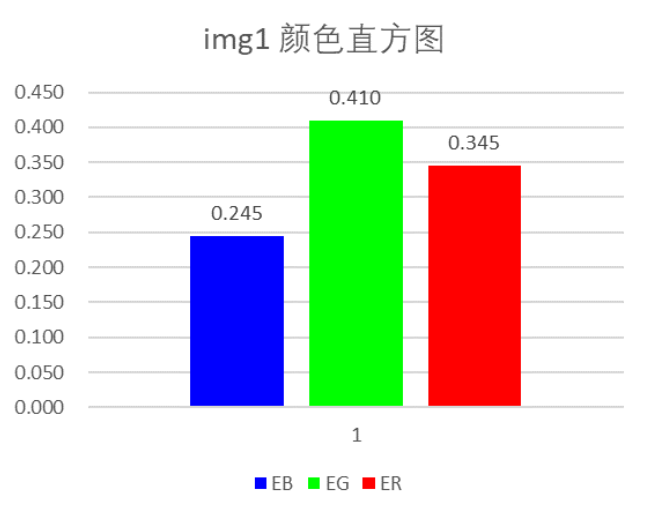
\includegraphics[width=13.5cm]{img/1-1.png}
\caption{img1的Canny边缘检测,阈值50-150,Sobel算子}
\label{1}
\end{figure}

\begin{figure}[htbp]
\centering
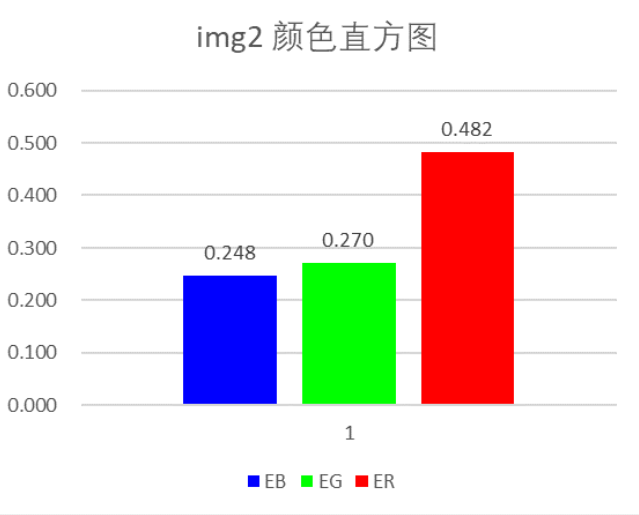
\includegraphics[width=13.5cm]{img/1-2.png}
\caption{img2的Canny边缘检测,阈值50-150,Sobel算子}
\label{2}
\end{figure}

\begin{figure}[htbp]
\centering
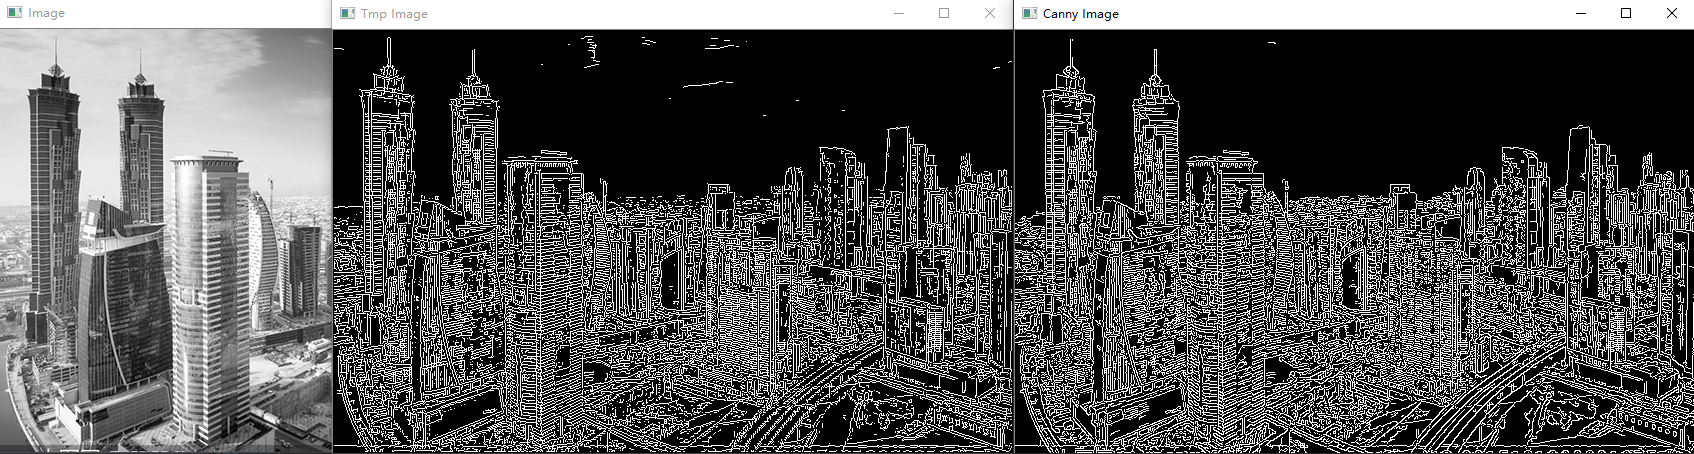
\includegraphics[width=13.5cm]{img/1-3.png}
\caption{img3的Canny边缘检测,阈值50-150,Sobel算子}
\label{3}
\end{figure}


\subsection{Canny算子的Canny检测}
我们的Canny检测与OpenCV中检测的效果对比如图\ref{4},\ref{5},\ref{6}所示。中间图示为我们构造的Canny检测函数效果,右图所示为对照图。阈值选取见图下注释。Canny算子计算出的赋值分量较小,因此需要仔细对阈值做调整,这也造成了边界模糊的问题。

\begin{figure}[htbp]
\centering
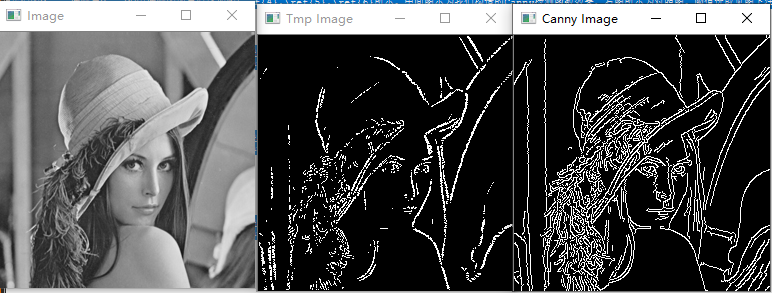
\includegraphics[width=13.5cm]{img/2-1.png}
\caption{img1的Canny边缘检测,阈值20-25,Canny算子}
\label{4}
\end{figure}

\begin{figure}[htbp]
\centering
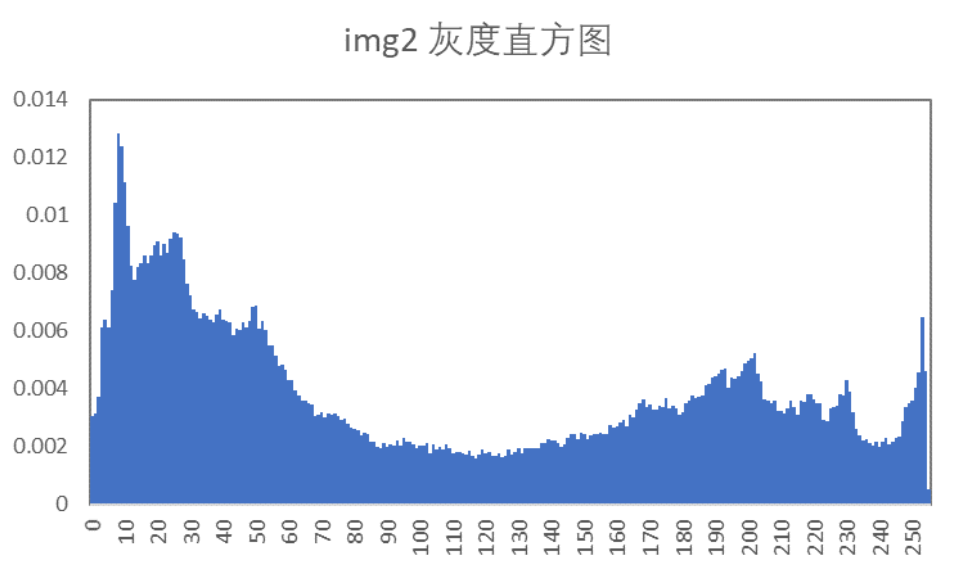
\includegraphics[width=13.5cm]{img/2-2.png}
\caption{img2的Canny边缘检测,阈值20-25,Canny算子}
\label{5}
\end{figure}

\begin{figure}[htbp]
\centering
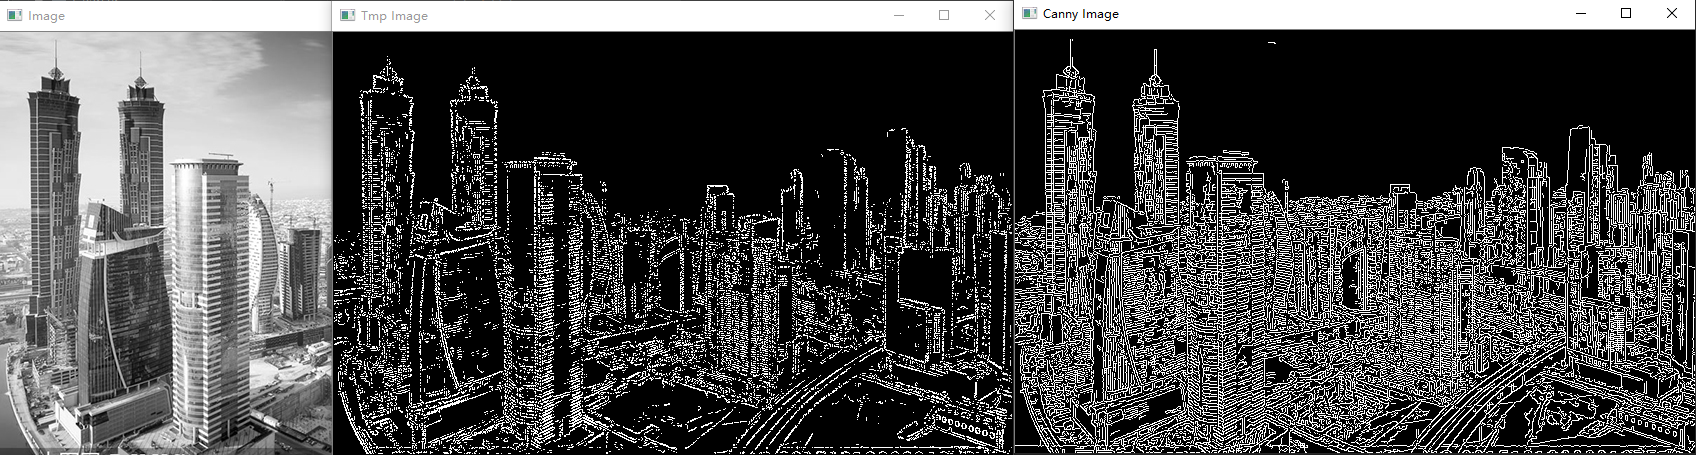
\includegraphics[width=13.5cm]{img/2-3.png}
\caption{img3的Canny边缘检测,阈值20-25,Canny算子}
\label{6}
\end{figure}


\subsection{Prewitt算子的Canny检测}
我们的Canny检测与OpenCV中检测的效果对比如图\ref{7},\ref{8},\ref{9}所示。中间图示为我们构造的Canny检测函数效果,右图所示为对照图。阈值选取见图下注释。由于Prewitt算子对上下左右四个邻点的权值在计算中削弱了,相比Sobel算子阈值也需要相应的调低。该算子产生的效果与Sobel的效果类似

\begin{figure}[htbp]
\centering
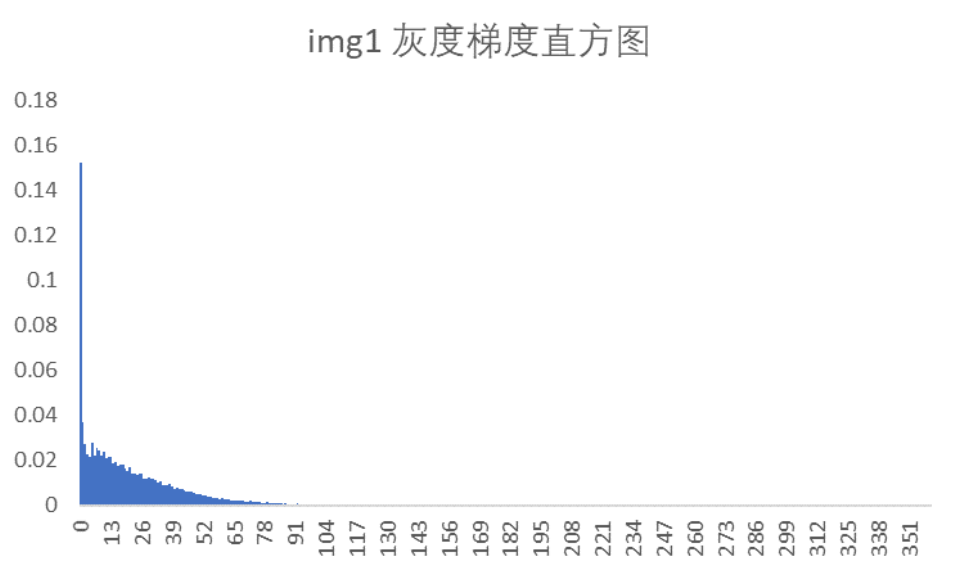
\includegraphics[width=13.5cm]{img/3-1.png}
\caption{img1的Canny边缘检测,阈值40-120,Prewitt算子}
\label{7}
\end{figure}

\begin{figure}[htbp]
\centering
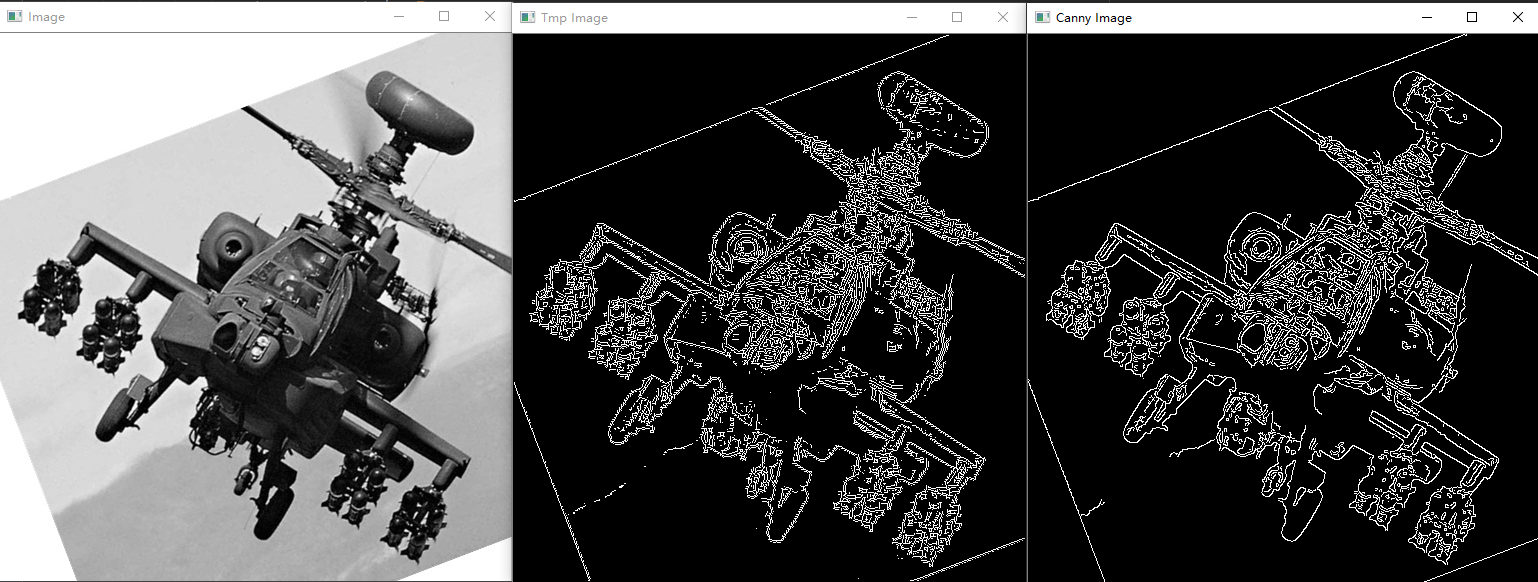
\includegraphics[width=13.5cm]{img/3-2.png}
\caption{img2的Canny边缘检测,阈值40-120,Prewitt算子}
\label{8}
\end{figure}

\begin{figure}[htbp]
\centering
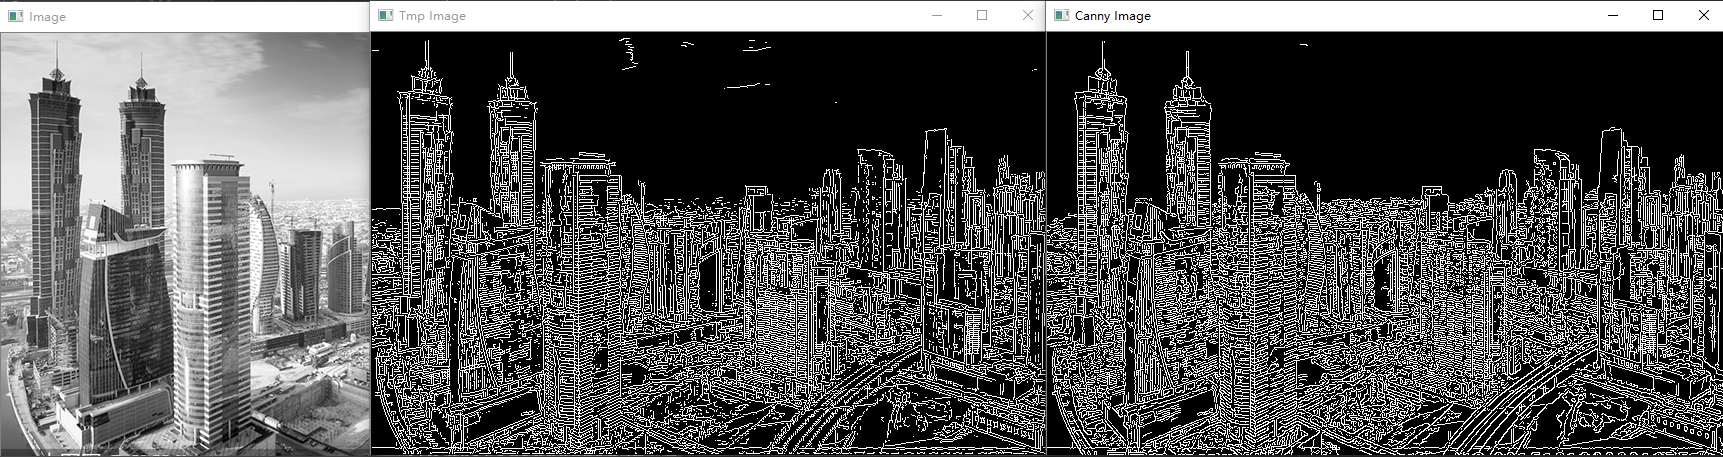
\includegraphics[width=13.5cm]{img/3-3.png}
\caption{img3的Canny边缘检测,阈值40-120,Prewitt算子}
\label{9}
\end{figure}

\section{实验总结}
\paragraph{概述}
本实验中,我们通过OpenCV实现了图像边缘检测的Canny算法。

\paragraph{感想}
通过本次实验的学习,我通过手动实现Canny算法的图像预处理、梯度计算、非极大值抑制和双阈值检测过程,对图像处理中的边缘检测的方法和思想有了更深的理解,也掌握了更多OpenCV和numpy矩阵操作的技巧。

\paragraph{问题}
本次实验中遇到的问题主要在技术层面。如我们需要妥善设置图像像素矩阵的数据类型,否则会产生溢出的问题。在计算幅度角度时,我们需要处理幅度X方向分量分母为0的问题。此外,我们还要对边缘检测中非极大值抑制的插值运算做好分类讨论。

\paragraph{创新}
本实验中除了Sobel算子外,还对Prewitt算子、Canny算子进行了实现,并且比照了其性能和边缘检测特征,在双阈值边缘检测中,我们用DFS的思想设计了算法,达到了较高的检测效率。

\end{document}

